\newpage
\part{Regression Diagnostics}
\section{Gauss-Markov Theorem}
The Gauss-Markov theorem states that in a linear regression model, where the errors
\begin{itemize}
	\item have expectation 0
	\item are uncorrelated
	\item have equal variances
\end{itemize}
the \textbf{Best Linear Unbiased Estimator (BLUE)} of the coefficients is given by the \textbf{Ordinary Least Square (OLS)} estimator.
\\ \ \\
Properties of the BLUE:
\begin{itemize}
	\item Unbiased: $E(\hat{\beta}) = \beta$
	\item Consistent: $n \uparrow$, $var(\hat{\beta}) \downarrow$  
	\item Efficient: $var(\hat{\beta}) < var(\tilde{\beta})$, it gives the \textbf{lowest variance} compared to other linear unbiased estimators. 
\end{itemize}

\section{Gauss-Markov Assumptions/Requirements}
The OLS estimator is the best linear unbiased estimator (BLUE), iff
\begin{figure}[H]
	\centering
	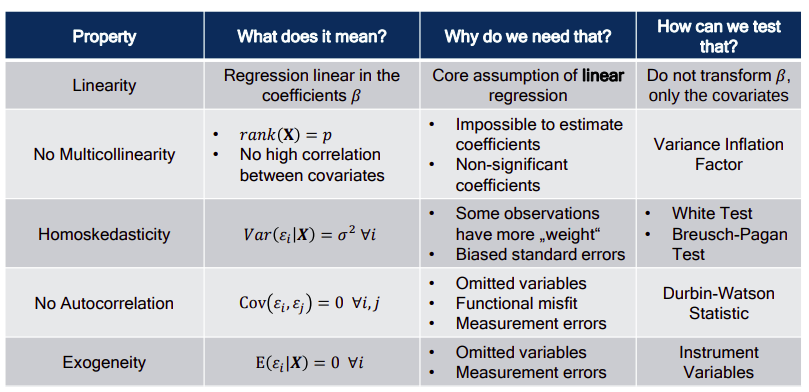
\includegraphics[width=0.9\textwidth]{gauss-markov.png}
\end{figure}
\subsection{Linearity}
\begin{itemize}
	\item Definition: Linear relationship in \textbf{coefficients} $\beta_i$.
	\item Why: core assumption of linear regression.
	\item Solution to non-linearity: Transform the \textbf{predictors or response}(logarithmic, interval-wise)
	\item Influence Factor: \textbf{outliers}. 
	
	Reasons for outlier: 
	\begin{itemize}
		\item error in recording the value
		\item point doesn't belong to the sample
		\item no error, it's an valid observation
	\end{itemize} 
	Solution to outlier:
	\begin{itemize}
		\item identify outliers $\rightarrow$ exclude 
		\item apply ''robust'' regression
	\end{itemize}
\end{itemize}

\subsection{No Multicollinearity}
\begin{itemize}
	\item Definition: \textbf{No} linear dependency between the \textbf{predictors} $X_i$
	
	$\rightarrow$ rank(X) = p (the data matrix has \textbf{full rank} = number of columns)
	
	$\rightarrow$ \textbf{No high correlation} between predictors (though full rank). 
	
	
	
	
	\item Testing: 
	\begin{itemize}
		\item \textbf{Correlation Coefficient} between predictor \textbf{pairs}
		\item \textbf{Variance Inflation Factor (VIF)}: correlation among \textbf{multiple predictors}
		$$VIF = \frac{1}{1-R^2_k}$$
		\paragraph{Interpretation of VIF} 
		
		When the predictor $X_k$ is set as the dependent variable, $R^2_k$ of the variance in the predictor $X_k$ can be explained by the rest of other predictors.
		
		eg: VIF = 10. $R^2_k$ = 90\%. 90\% of the variance in the predictor $X_k$ can be explained by the rest of other predictors.
		
		\paragraph{Rule} VIF $\uparrow$, Multicollinearity $\uparrow$. Remove predictor $X_k$ if $\mathbf{VIF >10}$
		
	\end{itemize}

	\item Consequences of Multicollinearity: Non-significance of the coefficients
	
	The coefficient has a small t-value/large p-value (can't reject $H_0$)
	\begin{itemize}
		\item small VIF: predictor $X_i$ is not related to response 
		
		$\rightarrow$ remove the variable $X_i$
		\item large VIF: predictor $X_i$ is highly correlated to some other predictors. 
		
		$\rightarrow$ \textbf{correlation matrix}: remove one of the highly correlated variables (near 1 or -1)
	\end{itemize}

	\item Example R-Interpretation: 
	\begin{figure}[H]
		\centering
		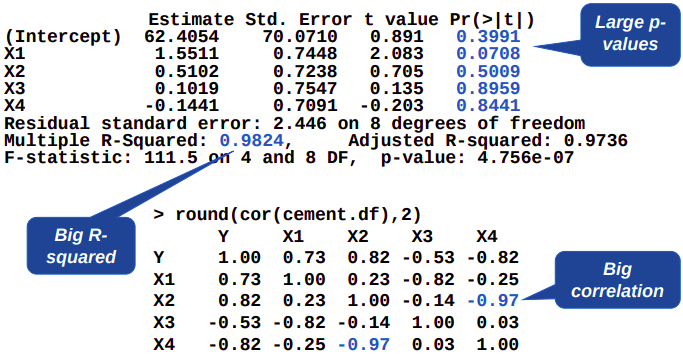
\includegraphics[width=0.6\textwidth]{vif1.png}
	\end{figure}
	\begin{figure}[H]
		\centering
		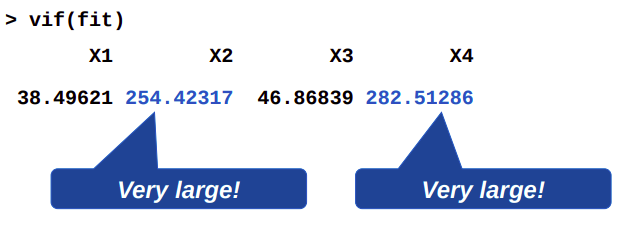
\includegraphics[width=0.6\textwidth]{vif2.png}
	\end{figure}
	large p-value, large VIF $\rightarrow$ high correlation among predictors. Call correlation matrix.
	
	Find out and remove one of the highly correlated predictors.
	\begin{figure}[H]
		\centering
		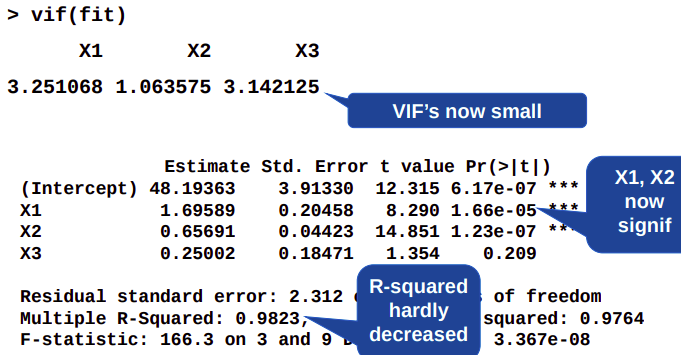
\includegraphics[width=0.6\textwidth]{vif3.png}
	\end{figure}
\end{itemize}

\subsection{Homoscedasticity}
\begin{itemize}
	\item Definition: \textbf{each residual $\sigma_i$} of predictor $X_i$ exhibit \textbf{constant} variance.
	
	$\rightarrow$ the spread of residual in different predictors remains nearly the same. 
	
	$\rightarrow$ no systematic development(grows larger/smaller) of residuals -- \textbf{Heteroscedasticity}
	
	\item Testing: 
	\begin{itemize}
		\item \textbf{Breusch-Pagan Test}
		\item \textbf{White Test}
		\begin{itemize}
			\item $H_0$: all variances $\sigma_i$ are equal (homoscedasticity)
			
			$H_1$: heteroscedasticity
			\item Distribution: $\chi^2$-Distribution
			\item reject $H_0$ if $p < \alpha$ 
		\end{itemize}
	\end{itemize}

	\item Consequence of Heteroscedasticity:
	\begin{itemize}
		\item estimated variance of coefficients $Var(\hat{\beta})$ is \textbf{biased}.
		\item OLS Estimator no longer efficient.
		\item Some predictors has more ''weight'' than others $\rightarrow$ higher sensitivity
	\end{itemize}
\end{itemize}

\subsection{No Autocorrelation}
\begin{itemize}
	\item Definition: no correlation between the $i^{th}$ and $j^{th}$ \textbf{overall residual}
	
	$\rightarrow$ $Cor(\varepsilon_i, \varepsilon_j) = 0$
	
	$\rightarrow$ \textbf{no pattern} of residuals should be observed over time, in case of \textbf{time series data}.
	
	
	\item Testing:
	
	The significance test of coefficients might say they are significant from 0. However, Autocorrelation detected. 
	\begin{itemize}
		\item visualize residuals against time
		\item \textbf{Durbin-Watson statistic [0,4]}: test for first-order autocorrelation
		$$DW = \frac{\Sigma_{i=2}^n (e_i - e_{i-1})^2}{\Sigma_{i=1}^n e_i^2}$$
		\paragraph{Interpretation of DW-statistic}
		\begin{itemize}
			\item DW = 2: \textbf{no} autocorrelation
			
			Rule of thumb: DW $\in$ [1.5, 2.5] $\rightarrow$ no serial correlation
			\item DW = 0: perfect \textbf{positive} autocorrelation
			\item DW = 4: perfect \textbf{negative} autocorrelation
		\end{itemize}
	\end{itemize}

	\item Consequences for autocorrelation:
	\begin{itemize}
		\item an important predictor is omitted (which explains the pattern over time)
		\item functional misfit 
		\item measurement error in predictors
	\end{itemize}

	\item Solution to autocorrelation: Model the missing predictor
	\begin{itemize}
		\item overall trend in time: t 
		\item dummy variable for seasonal indexes $Q_1$, $Q_2$, $Q_3$
		
		number of dummy variables: \textbf{number of choices -1} $\rightarrow$ avoid multicollinearity
	\end{itemize}

	Example Model: 
	$$y = \beta_0 + \beta_1\cdot t + \beta_2 \cdot Q_1 + \beta_3 \cdot Q_2 + \beta_4 \cdot Q_3$$
\end{itemize}

\subsection{Exogeneity}
\begin{itemize}
	\item Definition: the expected value of \textbf{residual vector} given all predictors is 0.
	
	$\rightarrow$ $E(\varepsilon|X) = 0$, $Cov(\varepsilon, X) = 0$
		
	
	\item Consequences for Endogeneity(not exogene):
	\begin{itemize}
		\item measurement error
		\item predictors and response effect each other mutually
		\item \textbf{important predictors are omitted} $\rightarrow$ bias in estimation of coefficients 
	\end{itemize}
	
	\item Testing for individual effects: \textbf{Lagrange Multiplier Test}, in R ''plmtest(model)''
	\begin{itemize}
		\item $H_0$: No individual effects
	\end{itemize}
	\item Testing for fixed or random effect model when Lagrange Multiplier Test fails: \textbf{Hausman Test}
	\begin{itemize}
		\item $H_0$: random effect estimator is consistent \& efficient $\rightarrow$ \textbf{random effect model}
		
		$H_1$: \textbf{fixed effect model} needed.
	\end{itemize}
	
	\item Solution to endogeneity due to omitted variable bias:
	
	according to types of data: 
	\paragraph{cross-section data} data observing many objects at the same time
		
	difficult to find out the confounding variables $\rightarrow$ \textbf{no solution}
	\paragraph{panel data} repeated observations on the same objects over time. Mostly unbalanced panel data, where some individuals are not recorded in all time period. 
	
	$\rightarrow$ individual-specific panel data structure
	
	$\rightarrow$ find out the omitted individual-specific effects on the response.
	
	Solution:
	\begin{itemize}
		\item \textbf{Fixed Effects Model}: 
		Individual/Entity-specific effects are \textbf{correlated} to other predictors
		
		$\rightarrow \lambda_i$ is constant, can be seen as \textbf{an additional intercept} for each individual $i$ in regression model. 
		
		$$y_{it} = (\beta_0 + \lambda_i) + \beta_1 x_{1it} + \beta_2 x_{2it} + \dots + \beta_k x_{kit} + \varepsilon_{it}$$
		
		Estimators for the fixed effect models: first differences, within, least square dummy variable
		\item \textbf{Random Effects Model}: 
		Individual/Entity-specific effects are \textbf{uncorrelated} to other predictors
		
		$\rightarrow \lambda_i$ is drawn independently, can be seen as \textbf{an element of residual} for each individual in regression model.
		$$y_{it} = \beta_0 + \beta_1 x_{1it} + \beta_2 x_{2it} + \dots + \beta_k x_{kit} + \underbrace{(\lambda_i + u_{it})}_{\varepsilon_{it}}$$	
	\end{itemize} 
\end{itemize}


